\appendix

\section{Visibility calculations \label{vis_appendix}}
*********Details of the vis preamble

\subsection{Basic integration for visibility calculations}
Recall equation~\ref{vis_equation} from Section~\ref{visibility}. In this equation, the quadratic limb darkening law is taken directly from \citet{Claret2004}:
\begin{equation}
   \frac{I(\mu)}{I(0)} = 1 - c_1 (1 - \mu) - c_2 (1 - \mu)^2
\end{equation}

Where $\mu = \sin\theta\cos\phi$ in spherical coordinates. Substituting equation~\ref{ld} into equation~\ref{vis_equation} yields:

\begin{equation}
\begin{split}
    V_{i,j} = \int_{\phi_1}^{\phi_2}  \int_{\theta_1}^{\theta_2} (1 - c_1 - c_2) \sin^2 \theta \cos \phi &+ (c_1 + 2 c_2) \sin^3 \theta \cos^2 \phi - c_2 \sin^4 \theta \cos^3 \phi \,\mathrm{d}\theta \, \mathrm{d}\phi
\end{split}
\end{equation}

We calculate this integral at every timestep for every region with $\phi_1$ and $\phi_2$ changing based on the region number and the rotational phase. $\theta_1$ and $\theta_2$ are constant in time, but different for boxes and longitudes as described in Section~\ref{visibilities}.

%This can be split into three separate integrals each with different degrees of $\sin\theta\cos\phi$. 
%These three answers are given below:
%
%\begin{equation}
%\begin{split}
%    V_{i,j}^0 =& (1 - c_1 - c_2) \frac{(\sin\phi_2 - \sin\phi_1)(\theta_2 - \theta_1 - \cos\theta_2\sin\theta_2 + \cos\theta_1\sin\theta_1)}{2}
%\end{split}
%\end{equation}
%
%\begin{equation}
%\begin{split}
%    V_{i,j}^1 =& (c_1 + 2 c_2) \frac{(9(\cos\theta_1 - \cos\theta_2) + \cos(3\theta_2) - \cos(3\theta_1))(\phi_2 - \phi_1 + \cos\phi_2\sin\phi_2 - \cos\phi_1\sin\phi_1)}{24}
%\end{split}
%\end{equation}
%
%\begin{equation}
%\begin{split}
%    V_{i,j}^2 =& - c_2 \frac{(12(\theta_2 - \theta_1) + 8(\sin(2\theta_1) - \sin(2\theta_2)) + \sin(4\theta_2) - \sin(4\theta_1))(9(\sin\phi_2 - \sin\phi_1) + \sin(3\phi_2) - \sin(3\phi_1))}{384}
%\end{split}
%\end{equation}
%
%Thus, the total visibility for a region $j$ at time $i$ is given by $V_{i,j}^0 + V_{i,j}^1 + V_{i,j}^2$.

\vspace{9mm}

\subsection{The transiting planet calculations \label{trans_appendix}}
The simplest case in which the planet is entirely contained within a box is:
\begin{equation}
	A_{occluded} = \pi r_p^2
\end{equation}

The planet can also be partially contained in a box in many ways, shown in Table~\ref{cases}. The sliver of the planet that is not within the box will be calculated and then extended to take care of all of the various cases. To do this, the area of a sector of a circle is found and then the triangle that is formed within it is subtracted. The sector is the combination of the light blue and yellow regions in Figure~\ref{eclipse}.
*******Make this eps
\begin{figure}[h]
	\centering
	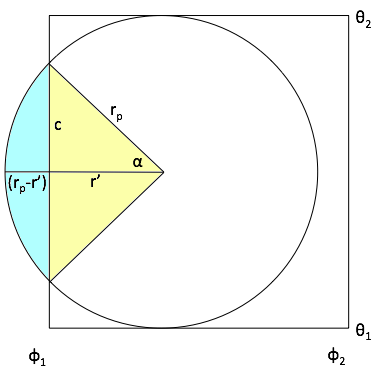
\includegraphics[width=.5\textwidth]{images/figure.png}
	\caption{Geometry of eclipse path visibility.}
	\label{eclipse}
\end{figure}

\begin{equation}
	A_{sector} = \frac{r_p \alpha^2}{2}
\end{equation}

where:

\begin{equation}
	\alpha = 2 \cos^{-1}\left(\frac{r^{\prime}}{r_p}\right)
\end{equation}

The area of the triangle is $cr^{\prime}$. $c$ is one half the length of the chord in the figure. $c$ can be found with the Pythagorean theorem. Knowing this, the area of the triangle becomes: 

\begin{equation}
	A_{triangle} = r^{\prime}\sqrt{r_p^2 - {r^{\prime}}^2}
\end{equation}

Finally, the area of the segment that indicates the part of the planet just over the border of the box is:

\begin{equation}
	A_{seg} = r_p^2 \cos^{-1}\left(\frac{r^{\prime}}{r_p}\right) - r^{\prime} \sqrt{r_p^2 - {r^{\prime}}^2}
\end{equation}

After completing the calculation of the area eclipsed by the planet, we multiply it by the average limb-darkened intensity in the containing box.


\begin{table}
	\caption{Subcases for planetary eclipse visibility}
	\label{cases}
	\begin{center}
	\renewcommand{\arraystretch}{1.2}
		\begin{tabular}{| m{.04\textwidth} | m{.24\textwidth} | m{.15\textwidth} |} %c means center justify, l left, r right
			\hline
			\textbf{Case}    & \textbf{Description} & \textbf{Area covered by planet in box}\\ %Separate with &, lines with \\
			\hline%horizontal line
			I      &   Planet is completely out of the box to the right                                                                      & 0                                                           \\ \hline
			II     &   Planet is completely out of the box to the left                                                                         & 0                                                           \\ \hline
			III    &   Planet is completely contained in the box                                                                              & $\pi r_p^2$                                         \\ \hline
			IV    &   Planet is partially off the right side of the box. Center is inside of the box                       & $\pi r_p^2 - A_{seg,l}$                     \\ \hline
			V     &   Planet is partially off the right side of the box. Center is outside of the box                     & $A_{seg}$                                          \\ \hline
			VI    &   Planet is partially off the left side of the box. Center is inside of the box                          & $\pi r_p^2 - A_{seg,r}$                     \\ \hline
			VII   &   Planet is partially off the left side of the box. Center is outside of the box                        & $A_{seg}$                                          \\ \hline
			VIII  &   Planet is partially off both sides of the box. Center is inside of the box                            & $\pi r_p^2 - A_{seg,r} - A_{seg,l}$ \\ \hline
			IX    &   Planet is partially off the right side of the box. Center is outside of the box to the left & $A_{seg,l1} - A_{seg,l2}$                \\ \hline
			X     &   Planet is partially off the left side of the box. Center is outside of the box to the right    & $A_{seg,r1} - A_{seg,r2}$               \\ \hline
		\end{tabular}
	\end{center}
\end{table}

\vspace{9mm}
\section{Results Continued \label{results_appendix}}
Using $A_{seg} $ and Table~\ref{cases}, a believable box-car transit model is produced. Note that $A_{seg,l}$ refers to a segment that is off the left side of a box relative to the center of the planet and likewise for $A_{seg,r}$. The subscripts $A_{seg,r1}$ and $A_{seg,r2}$ and likewise for the left refer to cases where there are two portions off one side of a box relative to the center of the planet. Limb darkening must also be included in order to give a better approximation to the actual shape of a real transit. This is introduced in the visibility rather than in the model flux calculation. This is okay because $\fmod = V_{i,j} b{j}$. If limb-darkening were calculated during every flux calculation of every chi-squared call during the Amoeba algorithm run, it would require much more operational complexity in the code. However, limb-darkening can be calculated before the many chi-squared calls via the Amoeba algorithm and and avoid this.  The geometric analysis of the transit and limb darkening is continued in the next section.


The top two plots show the brightness map as it appears on a projected star. The left map shows the input brightness values to the system for the production of the light curves. The map on the right shows the average recovered brightness over 24 windows that were modeled over the 30 day data set. Each window was 14 days wide and the increment between start times of the windows was 0.3 days. The next two plots show the box and stripe brightness values as a function of window. The region number corresponds to the tuple defined in Section~\ref{model_flux}, Equation~\ref{tuple}. The hue represents the brightness value and should be the same scale for all four of these pictures reporting brightness values. Each column in these plots is one window. The far right column (separated by a line) shows the input brightness value for that region. The next plot shows the standard deviation of the average recovered value in a region compared to the input value for that region. The boxes are to the left of the black line, and the stripes are to the right. Note that the region numbers are the same as in the box and stripe brightness plots above. The final plot is the fit to the synthetic light curve. This plot shows the entire month of data that was created. Every model is over-plotted. The model light curves are shown in black while the synthetic light curves are the red points. Note that models overlap significantly due to the fact that the start times are only 0.3 days (~$\frac{1}{5}$ orbital phase units) apart per window while the window length is 14 days.

\clearpage
\begin{figure}
	\includegraphics[width=1\textwidth]{images/1b_14_page.eps}
	\caption{Diagnostic plots for synthetic starspot system recovery.}
	\label{page_1b}
\end{figure}
\clearpage
\begin{figure}
	\includegraphics[width=1\textwidth]{images/1b_14_transit.eps}
	\caption{Each of the transits for the month of synthetic data. The transits are in order as English is read. Each transit plot shows the synthetic data in red points with every relevant model overlaid in grey lines.}
	\label{transits_1b}
\end{figure}

\clearpage
\begin{figure}
	\includegraphics[width=1\textwidth]{images/1b_1s_14_page.eps}
	\caption{Diagnostic plots for synthetic starspot system recoverys.}
	\label{page_1b_1s}
\end{figure}
\clearpage
\begin{figure}
	\includegraphics[width=1\textwidth]{images/1b_1s_14_transit.eps}
	\caption{Each of the transits for the month of synthetic data. The transits are in order as English is read. Each transit plot shows the synthetic data in red points with every relevant model overlaid in grey lines.}
	\label{transits_1b_1s}
\end{figure}

\clearpage
\begin{figure}
	\includegraphics[width=1\textwidth]{images/2b_14_page.eps}
	\caption{Diagnostic plots for synthetic starspot system recovery.}
	\label{page_2b}
\end{figure}
\clearpage
\begin{figure}
	\includegraphics[width=1\textwidth]{images/2b_14_transit.eps}
	\caption{Each of the transits for the month of synthetic data. The transits are in order as English is read. Each transit plot shows the synthetic data in red points with every relevant model overlaid in grey lines.}
	\label{transits_2b}
\end{figure}

\clearpage
\begin{figure}
	\includegraphics[width=1\textwidth]{images/2b_1s_14_page.eps}
	\caption{Diagnostic plots for synthetic starspot system recovery.}
	\label{page_2b_1s}
\end{figure}
\clearpage
\begin{figure}
	\includegraphics[width=1\textwidth]{images/2b_1s_14_transit.eps}
	\caption{Each of the transits for the month of synthetic data. The transits are in order as English is read. Each transit plot shows the synthetic data in red points with every relevant model overlaid in grey lines.}
	\label{transits_2b_1s}
\end{figure}

\clearpage
\begin{figure}
	\includegraphics[width=1\textwidth]{images/2b_2s_14_page.eps}
	\caption{Diagnostic plots for synthetic starspot system recovery..}
	\label{page_2b_2s}
\end{figure}
\clearpage
\begin{figure}
	\includegraphics[width=1\textwidth]{images/2b_2s_14_transit.eps}
	\caption{Each of the transits for the month of synthetic data. The transits are in order as English is read. Each transit plot shows the synthetic data in red points with every relevant model overlaid in grey lines.}
	\label{transits_2b_2s}
\end{figure}

\clearpage
\begin{figure}
	\includegraphics[width=1\textwidth]{images/3b_1s_14_page.eps}
	\caption{Diagnostic plots for synthetic starspot system recovery.}
	\label{page_3b_1s}
\end{figure}
\clearpage
\begin{figure}
	\includegraphics[width=1\textwidth]{images/3b_1s_14_transit.eps}
	\caption{Each of the transits for the month of synthetic data. The transits are in order as English is read. Each transit plot shows the synthetic data in red points with every relevant model overlaid in grey lines.}
	\label{transits_3b_1s}
\end{figure}